\documentclass[a4paper,9pt]{scrartcl}
\usepackage{amssymb, amsmath} % needed for math
\usepackage[utf8]{inputenc} % this is needed for umlauts
\usepackage[ngerman]{babel} % this is needed for umlauts
\usepackage[T1]{fontenc}    % this is needed for correct output of umlauts in pdf
\usepackage[margin=2.0cm]{geometry} %layout
\usepackage{hyperref}   % links im text
\usepackage{enumerate}  % for advanced numbering of lists
\usepackage{color}
\usepackage{framed}
\usepackage{float}
\usepackage{caption}
\usepackage{csquotes}
\usepackage[hang]{subfigure}
\usepackage[pdftex,final]{graphicx}
\usepackage{pgfplots}
\usepackage{tikz}
\usepackage{tikzscale}
\usetikzlibrary{shapes, calc, shapes, arrows}
\DeclareMathOperator{\sigmoid}{sigmoid}

\newcommand\titleText{Kreativität im maschinellen Lernen}
\title{\vspace{-5ex}\titleText\vspace{-7ex}}
\author{}
\date{}
\hypersetup{
  pdfauthor   = {Martin Thoma},
  pdfkeywords = {Machine Learning, Art, Creativity},
  pdftitle    = {\titleText}
}

\usepackage{fancyhdr}
\pagestyle{fancy}
\fancyhead{}
\fancyfoot{}
\fancyhead[L]{Referat vom 15.01.2016}
\fancyhead[R]{Martin Thoma}
\renewcommand{\headrulewidth}{0.4pt}

\makeatletter
\let\ps@plain\ps@fancy
\makeatother

%%%%%%%%%%%%%%%%%%%%%%%%%%%%%%%%%%%%%%%%%%%%%%%%%%%%%%%%%%%%%%%%%%%%%
% Custom definition style, by                                       %
% http://mathoverflow.net/questions/46583/what-is-a-satisfactory-way-to-format-definitions-in-latex/58164#58164
%%%%%%%%%%%%%%%%%%%%%%%%%%%%%%%%%%%%%%%%%%%%%%%%%%%%%%%%%%%%%%%%%%%%%
\makeatletter
\newdimen\errorsize \errorsize=0.2pt
% Frame with a label at top
\newcommand\LabFrame[2]{%
    \fboxrule=\FrameRule
    \fboxsep=-\errorsize
    \textcolor{FrameColor}{%
    \fbox{%
      \vbox{\nobreak
      \advance\FrameSep\errorsize
      \begingroup
        \advance\baselineskip\FrameSep
        \hrule height \baselineskip
        \nobreak
        \vskip-\baselineskip
      \endgroup
      \vskip 0.5\FrameSep
      \hbox{\hskip\FrameSep \strut
        \textcolor{TitleColor}{\textbf{#1}}}%
      \nobreak \nointerlineskip
      \vskip 1.3\FrameSep
      \hbox{\hskip\FrameSep
        {\normalcolor#2}%
        \hskip\FrameSep}%
      \vskip\FrameSep
    }}%
}}
\definecolor{FrameColor}{rgb}{0.25,0.25,1.0}
\definecolor{TitleColor}{rgb}{1.0,1.0,1.0}

\newenvironment{contlabelframe}[2][\Frame@Lab\ (cont.)]{%
  % Optional continuation label defaults to the first label plus
  \def\Frame@Lab{#2}%
  \def\FrameCommand{\LabFrame{#2}}%
  \def\FirstFrameCommand{\LabFrame{#2}}%
  \def\MidFrameCommand{\LabFrame{#1}}%
  \def\LastFrameCommand{\LabFrame{#1}}%
  \MakeFramed{\advance\hsize-\width \FrameRestore}
}{\endMakeFramed}
\newcounter{definition}
\newenvironment{definition}[1]{%
  \par
  \refstepcounter{definition}%
  \begin{contlabelframe}{Definition \thedefinition:\quad #1}
 \noindent\ignorespaces}
{\end{contlabelframe}}
\makeatother
%%%%%%%%%%%%%%%%%%%%%%%%%%%%%%%%%%%%%%%%%%%%%%%%%%%%%%%%%%%%%%%%%%%%%
% Begin document                                                    %
%%%%%%%%%%%%%%%%%%%%%%%%%%%%%%%%%%%%%%%%%%%%%%%%%%%%%%%%%%%%%%%%%%%%%
\begin{document}
\maketitle
\begin{definition}{Machine Learning (ML) nach Tom Mitchell}
A computer program is said to learn from \textbf{experience}~$\mathbf{E}$ with
respect to some class of \textbf{tasks}~$\mathbf{T}$ and \textbf{performance
measure}~$\mathbf{P}$, if its performance at tasks in~$T$, as measured by~$P$,
improves with experience~$E$.
\end{definition}

\begin{figure}[H]
\centering
\subfigure[Aufbau eines künstlichen Neurons. Die Eingabesignale werden mit $x_i \in \mathbb{R}$ bezeichnet; $w_i \in \mathbb{R}$ heißen \textit{Gewichte} und müssen gelernt werden. Jedes Eingabesignal wird mit seinem Gewicht multipliziert. Die Produkte werden aufsummiert. Dann wird die sog. \textit{Aktivierungsfuntkion} $i$ angewendet.]{
  \label{fig:artificial-neuron}
  \includegraphics[width=0.45\linewidth]{neuron.tikz}
}%
\subfigure[Eine einfaches Feed-Forward Neuronales Netz. Die 5~Eingabeneuronen sind rot, die 2~Bias-Neuronen sind Grau, die 3~Hidden-Neuronen sind Grün und das einzelne Ausgabeneuron ist Blau. Dieses 3-schichtige Modell hat $6 \cdot 4 + 4 \cdot 1 = 28$ Kanten. Für jede Kante muss ein Gewicht $w_{ij} \in \mathbb{R}$ gelernt werden.]{
  \label{fig:feed-forward-nn}
  \includegraphics[width=0.45\linewidth]{feed-forward-nn.tikz}
}

\subfigure[Beispiele für Aktivierungsfuntkionen $\varphi: \mathbb{R} \rightarrow \mathbb{R}$]{
  \label{fig:artificial-neuron}
  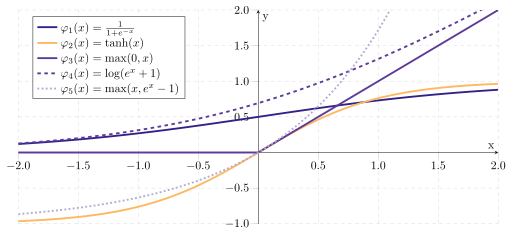
\includegraphics[width=0.9\linewidth]{activation-functions.tikz}
}%

\caption{Neuronale Netze basieren auf einfachen Einheiten, welche zu komplexen Netzwerken verschaltet werden können. Diese können mittels \textit{Gradientenabstieg} automatisch trainiert werden.}
\label{fig:neural-style}
\end{figure}

\begin{definition}{Convolutional Neural Network (CNN)}
Ein CNN ist ein neuronales Netz, welches keine vollverbundenen Schichten hat
sondern die Gewichte von Bildfiltern lernt.
\end{definition}

\begin{definition}{Rekurrentes Neuronale Netz (RNN)}
Ein RNN ist ein neuronales Netz, welches Kanten hat, die zeitlich versetzt
wieder als Eingabe genutzt werden.
\end{definition}

CNNs können sehr effektiv für Bilder eingesetzt werden, RNNs können zur
Behandlung von Sequenzen verwendet werden. Insbesondere können beliebig lange
Eingabesequenzen genutzt werden und unabhängig von der Eingabe beliebig lange
Ausgaben erzeugt werden.

\begin{definition}{Google DeepDream}
Google DeepDream ist eine Abwandlung einer Technik zur Analyse der gelernten
Gewichte.
\end{definition}

\section*{Quellen}
Alle Quellen und eine detailierte Beschreibung der Verfahren sind unter\\
\url{https://github.com/MartinThoma/seminar-art-in-machine-learning} sowie im arXiv unter\\
\enquote{Creativity in Machine Learning} --- \url{http://arxiv.org/abs/1601.03642} ---
zu finden.

\end{document}
